%%%%%%%%%%%%%%%%%%%%%%%%%%%%%%%%%%%%%%%%%%%%
% DMECS Dissertation Research Plan
% LaTeX Template
% Version 1.0 (November 2026), adapted from MESCC Dissertation template
%
% [Dissertation Planned Title here]
%
% Author: Student Name
% Supervisor: Supervisor Name
% Co-supervisor: Co-supervisor Name (if applicable)
% Course: Master's in Critical Computing Systems Engineering
% ISEP - School of Engineering, Polytechnic of Porto
% Creation Date: [Insert creation date here]
%
% This document uses the DMESC-style.sty template
%%%%%%%%%%%%%%%%%%%%%%%%%%%%%%%%%%%%%%%%%


%----------------------------------------------------------------------------------------
%	DOCUMENT CONFIGURATIONS
%----------------------------------------------------------------------------------------

\documentclass[
	11pt, % The default document font size, options: 10pt, 11pt, 12pt
	%oneside, % Two side (alternating margins) for binding by default, uncomment to switch to one side (for drafting/reading purposes)
	english, % english for English;
	%portuguese, % for Portuguese; delete temporary files if you change language (e.g. 'make clean; make')
	%singlespacing, % Single line spacing, alternatives: onehalfspacing or doublespacing (for drafting/reading purposes)
	onehalfspacing, % AMB: Specified by the ISEP template guidelines.
	%draft, % Uncomment to enable draft mode (no pictures, no links, overfull hboxes indicated)
	nolistspacing, % If the document is onehalfspacing or doublespacing, uncomment this to set spacing in lists to single
	%liststotoc, % Uncomment to add the list of figures/tables/etc to the table of contents (not recommended)
	%toctotoc, % Uncomment to add the main table of contents to the table of contents (not recommended)
	parskip, % Add space between paragraphs (recommended)
	%nohyperref, % Uncomment to not load the hyperref package (not recommended)
	nohyperreflinkcolor, % hyperref links are not colored (comment to color links, for example to produce an electronic-only version)
	headsepline, % Uncomment to get a line under the header
]{dmesc-style} % The class file specifying the document structure


%----------------------------------------------------------------------------------------
%	ADDITIONAL PACKAGES AND CUSTOM PACKAGE CONFIGURATIONS
%----------------------------------------------------------------------------------------

% In this section you can add any additional packages you need to use in your 
% dissertation.
%   - Do not modify the style of the document, as it is already configured in
%     the dmesc-style.cls file.
%   - Do not add any packages that are already included in the dmesc-style.cls file,
%     as this may cause conflicts.

% You can also configure the packages here, but do not modify the style of
% the document.

% Define TIKZ libraries to be used in the document (uncomment if needed)
%\usetikzlibrary{arrows} % Required for fancy arrows in TiKZ graphics (can be removed if not used)


%----------------------------------------------------------------------------------------
%	CITATION STYLE CONFIGURATION
%----------------------------------------------------------------------------------------

% Next you have examples of admissable citation styles; we recomend using the
% authoryear-comp citation style (which resembles Harvard).
% Don't forget to only uncomment one.

% AMB: According to ISEP dissertation guidelines you should use the authoryear-comp
% citation style (e.g. (Buendía, 1860), (Buendía 1910, Arcadio 1940)). Do not use the
% numeric citation style (e.g. [1], [1-3]) or the alphabetic citation style
% (e.g. [Buendía10], [Buendía10, Arcadio40]).

% authoryear-comp: recommended citation style (e.g. (Buendía, 1860), (Buendía 1910, Arcadio 1940))
\usepackage[style=authoryear-comp,backend=biber]{biblatex} % Bibtex backend with the authoryear-comp citation style (authoryear citations, bibliography ordered alphabetically)

% numeric citation style (e.g. [1], [1-3])
%\usepackage[style=numeric-comp,sorting=none,backend=biber]{biblatex} % Bibtex backend with the numeric-comp citation style (numeric citations, bibliography ordered by appearance)

% alphabetic citation style (e.g. [Buendía10], [Buendía10, Arcadio40])
%\usepackage[style=alphabetic,sorting=none,backend=biber]{biblatex} % Bibtex backend with the alphabetic citation style (alphabetic citations, bibliography ordered by appearance)


%----------------------------------------------------------------------------------------
%	SIMPLE PATCH TO ADAPT THE TITLE PAGE TO THE DISSERTATION RESEARCH PLAN
%----------------------------------------------------------------------------------------
\patchcmd{\maketitlepage}{\evallabel:}{}{}{}
\patchcmd{\maketitlepage}{\presidentlabel:}{}{}{}
\patchcmd{\maketitlepage}{\presidentname}{}{}{}
\patchcmd{\maketitlepage}{\memberslabel:}{}{}{}
\patchcmd{\maketitlepage}{\committee}{}{}{}
\patchcmd{\maketitlepage}{\externalsupervisor}{}{}{}

% Automatic Disclaimer configuration per language
\iflanguage{portuguese}{
    \renewcaptionname{portuguese}{\dissertationdisclamer}{Plano de Investigação da Dissertação \\ Mestrado em Engenharia de Sistemas Computacionais Críticos}

}{
		\renewcaptionname{english}{\dissertationdisclamer}{Dissertation Research Plan \\ Master's degree in Critical Computing Systems Engineering}
}


%----------------------------------------------------------------------------------------
%	GLOSSARY CONFIGURATION
%----------------------------------------------------------------------------------------
\addbibresource{mainbibliography.bib} % The filename of the bibliography

\makeglossaries % build the glossary


%----------------------------------------------------------------------------------------
%	THESIS INFORMATION
%----------------------------------------------------------------------------------------

% Your thesis title, this is used in the title, print it elsewhere with \ttitle
\thesistitle{Dissertation Planned Title} 

% Your thesis subtitle, this is used in the title, print it elsewhere with \tsubtitle, comment line if not existing
\thesissubtitle{Subtitle (if exists)}

% Your name, this is used in the title page, print it elsewhere with \authorname
\author{Candidate Full Name} 

% Your supervisor's name, this is used in the title page, print it elsewhere with \supname
\supervisor{Full Name} 

% Your co-supervisor's name, this is used in the title page, print it elsewhere with \cosupname (comment, if no co-supervisor)
\cosupervisor{Full Name (if exists)} 

% Please define up to 6 keywords that better describe your work, print it elsewhere with \keywordnames
\keywords{Keyword1, ..., Keyword6} 

% Thesis date, print it elsewhere with \tdate
\thesisdate{Porto, \today} 

\hypersetup{pdftitle=\ttitle} % Set the PDF's title to your title
\hypersetup{pdfauthor=\authorname} % Set the PDF's author to your name
\hypersetup{pdfkeywords=\keywordnames} % Set the PDF's keywords to your keywords


%----------------------------------------------------------------------------------------
%	THE CONTENT OF THE DOCUMENT BEGINS HERE
%----------------------------------------------------------------------------------------

\begin{document}


%----------------------------------------------------------------------------------------
%	FRONT MATTER
%----------------------------------------------------------------------------------------

% Include the frontmatter of your thesis here

% we include the glossary here (frontmatter is included with \input, so this command is as if it was in main.tex)
%All acronyms must be written in this file.
\newacronym{RTS}{RTS}{Real-Time System}
\newacronym{GPOS}{GPOS}{General Purpose Operating System}
\newacronym{RTOS}{RTOS}{Real-Time Operating System}
\newacronym{PGF}{PGF}{Portable Graphics Format}
\newacronym{X}{X}{X}

\frontmatter % Use roman page numbering style (i, ii, iii, iv...) for the pre-content pages

\pagestyle{plain} % Default to the plain heading style until the thesis style is called for the body content

%----------------------------------------------------------------------------------------
%	TITLE PAGE
%----------------------------------------------------------------------------------------

	
\maketitlepage


%----------------------------------------------------------------------------------------
%	STATEMENT of INTEGRITY
%----------------------------------------------------------------------------------------

\integritystatement

%----------------------------------------------------------------------------------------
%	ABSTRACT PAGE
%----------------------------------------------------------------------------------------

\begin{abstract}

% here you put the abstract in the main language of the work.

This document contains the main formatting rules to be applied in the writing of the Dissertation Plan of the Master in Critical Computing Systems Engineering, of the Department of Computer Engineering, of ISEP. The rules presented here form a set of best practices recommended for writing the document. However, it is recommended to discuss these and other aspects with the respective supervisor.

The rules to be followed are presented regarding the format of the paper to be used, how the document is organized, general rules for formatting the text, formatting tables and figures, inserting bibliographic references in the text and presenting bibliographic references.

The document must contain an abstract in Portuguese and English. The abstract in the  language of the document should come first and not exceed 200 words or one A4 page. The abstract in the other language should be an extended one, not exceeding 1000 words or two A4 pages.

This document was adapted from the master's dissertation model in Informatics Engineering at ISEP, originally prepared by Professor Fátima Rodrigues (DEI/ISEP).

After the abstract, it is mandatory to place the main keywords of the theme of the work, with a maximum of 6 keywords being allowed. Keywords are defined in the \emph{THESIS INFORMATION} block of the \file{main.tex} file.

\end{abstract}

\begin{abstractotherlanguage}
% here you put the abstract in the "other language": English, if the work is written in Portuguese; Portuguese, if the work is written in English.

Este documento contém as principais regras de formatação a aplicar na redação do Plano de Dissertação do Mestrado em Engenharia de Sistemas Computacionais Críticos, do Departamento de Engenharia Informática, do ISEP. As regras aqui apresentadas formam um conjunto de boas práticas recomendadas para escrever o documento. No entanto, é recomendável discutir esses e outros aspetos com o respetivo supervisor. 

São apresentadas as regras a serem seguidas quanto ao formato a ser utilizado, a organização do documento, as regras gerais de formatação do texto, formatação de tabelas e figuras, inserção de referências bibliográficas no texto e apresentação de referências bibliográficas.

O documento deve conter o resumo em português e em inglês. O resumo no idioma do documento deve vir primeiro e não deve exceder 200 palavras ou uma página A4. O resumo no outro idioma deve ser estendido, não excedendo 1000 palavras ou duas páginas A4.

Este documento foi adaptado do modelo de dissertação de mestrado em Engenharia Informática do ISEP, originalmente elaborado pela Professora Fátima Rodrigues (DEI/ISEP).

Para alterar a língua basta ir às configurações do documento no ficheiro \file{main.tex} e alterar para a língua desejada ('english' ou 'portuguese')\footnote{Alterar a língua requer apagar alguns ficheiros temporários; O target \keyword{clean} do \keyword{Makefile} incluído pode ser utilizado para este propósito.}. Isto fará com que os cabeçalhos incluídos no template sejam traduzidos para a respetiva língua.

\end{abstractotherlanguage}


%----------------------------------------------------------------------------------------
%	LIST OF CONTENTS/FIGURES/TABLES PAGES
%----------------------------------------------------------------------------------------

\tableofcontents % Prints the main table of contents

\listoffigures % Prints the list of figures

\listoftables % Prints the list of tables

\iflanguage{portuguese}{
\renewcommand{\listalgorithmname}{Lista de Algor\'itmos}
}
\listofalgorithms % Prints the list of algorithms
%\addchaptertocentry{\listalgorithmname}


\renewcommand{\lstlistlistingname}{List of Source Code}
\iflanguage{portuguese}{
\renewcommand{\lstlistlistingname}{Lista de C\'odigo}
}
\lstlistoflistings % Prints the list of listings (programming language source code)
%\addchaptertocentry{\lstlistlistingname}


%----------------------------------------------------------------------------------------
%	ABBREVIATIONS
%----------------------------------------------------------------------------------------
\begin{abbreviations}{ll} % Include a list of abbreviations (a table of two columns)
\textbf{LAH} & \textbf{L}ist \textbf{A}bbreviations \textbf{H}ere\\
\textbf{WSF} & \textbf{W}hat (it) \textbf{S}tands \textbf{F}or\\
\end{abbreviations}

%----------------------------------------------------------------------------------------
%	SYMBOLS
%----------------------------------------------------------------------------------------

\begin{symbols}{lll} % Include a list of Symbols (a three column table)

% [Note: Although acronyms and symbols are defined in this section, they should also be defined at least the first time used in the dissertation body.]

$a$ & distance & \si{\meter} \\
$P$ & power & \si{\watt} (\si{\joule\per\second}) \\
%Symbol & Name & Unit \\

\addlinespace % Gap to separate the Roman symbols from the Greek

$\omega$ & angular frequency & \si{\radian} \\

\end{symbols}



%----------------------------------------------------------------------------------------
%	ACRONYMS
%----------------------------------------------------------------------------------------

\newcommand{\listacronymname}{List of Acronyms}
\iflanguage{portuguese}{
\renewcommand{\listacronymname}{Lista de Acr\'onimos}
}

%Use GLS
\glsresetall
\printglossary[title=\listacronymname,type=\acronymtype,style=long]

%----------------------------------------------------------------------------------------
%	DONE
%----------------------------------------------------------------------------------------

\mainmatter % Begin numeric (1,2,3...) page numbering
\pagestyle{thesis} % Return the page headers back to the "thesis" style



%----------------------------------------------------------------------------------------
%	MAIN BODY
%----------------------------------------------------------------------------------------

% Include the chapters of the thesis as separate folder for each chapter
% Uncomment the lines as you write the chapters

% Chapter 1
% 
\chapter{Introduction} % Main chapter title
\label{chap:Chapter1} % For referencing the chapter elsewhere, use Chapter~\ref{Chapter1}


%-------------------------------------------------------------------------------
%---------
%
\section{Writing guidelines} 
\label{sec:chap1_guidelines} %For referencing this section elsewhere, use Section~\ref{sec:chap1_guidelines}

This chapter presents some recommendations to follow in the structuring and formatting of the dissertation research plan.

The purpose of writing a research plan is, in essence, to document the work developed and highlight its importance. The author must follow the best writing rules, that is, respect grammatical and spelling rules, and correctly organize the text in order to make the message to be conveyed clear. 

The language used must be rigorous, scientific and without colloquial expressions. If in Portuguese, the document must be written using the rules of the new Orthographic Agreement that took effect in January 2009. If in English, the document should follow the rules of the United Kingdom variant. 

Automatic spelling correction must be complemented by consulting grammars and glossaries.

\section{Document structure}

The structure of the dissertation is normally divided into three main parts: Introduction, State of the art and Research Plan.

The Introduction should contain the following subsections:
\begin{itemize}
    \item Background and Motivation (context, relevance and motivation)
    \item Problem Statement (the problem, gaps and definition of scope)
    \item Goal and Objectives (the main goal and its measurable objectives)
    \item Research Questions (the questions that will guide the research)
    \item Privacy and Ethics (see Section 1.4)
    \item Use of AI Tools (see Section 1.5)
    \item Document Structure (brief description of the following chapters)
\end{itemize}

The main Body of the document includes the survey of the state of the art carried out, normally placed in the chapter following the Introduction. The survey of the state of the art should not be too exhaustive, focusing on the specific topics addressed in the document. This state of the art is intended to be updated during the writing of the dissertation. The structure of this chapter should be discussed with the supervisor.

An optional chapter can be added, with initial work already performed, such as a proposed approach and/or preliminary results.

Finally, a Research Plan chapter needs to be provided, with information on the work to be performed during the 2\textsuperscript{nd} semester.

\begin{itemize}
    \item the methodology of the work to be developed (summary of the approach, methods, prototypes, experimentation, etc.);
    \item how the results are going to be evaluated to allow the research questions to be answered;
    \item timeline of activities for the second semester.
\end{itemize}

\subsection{Contents checklist}

Table~\ref{tab:checklist} provides a list to check the contents of the document. 

\begin{table}[H]
\caption{Contents checklist.}
\label{tab:checklist}
\centering
\begin{tabular}{l l l}
\toprule
\tabhead{Description} & \tabhead{Mandatory?} & \tabhead{Page numbers} \\
\midrule
First page (template first page)&Yes&None\\
Statement of Integrity&Yes&Roman\\
Portuguese abstract (Resumo)&Yes&Roman\\
English abstract &Yes&Roman\\
Table of Contents&Yes&Roman\\
List of Figures&Yes&Roman\\
List of Tables&Yes&Roman\\
Acronyms and Symbols&Yes&Roman\\
Introduction&Yes&Arabic\\
State of the art&Yes&Arabic\\
Preliminary Results&No&Arabic\\
Research Plan&Yes&Arabic\\
References&Yes&Arabic\\
Annexes and appendices&No&Arabic\\

\bottomrule\\
\end{tabular}
\end{table}


\section{Formatting}

The document can be written in Portuguese or English. The minimum number of pages is 30 and the maximum is 60. Complementary documentation may be added in the form of annexes, never exceeding 90 pages in total (including the main text of the dissertation). 

Please follow the margins and fonts  defined in this template. The font size should be 11pt. The document should be printed double sided.

Please note that the graphic appearance and formatting are not a substitute for well-organized writing and a clear presentation of ideas. 

Please refer to the annex~\ref{AppendixA} for details about this template, how to format the document and insert citations, figures, tables, equations and other elements.

\section{Privacy and ethics}
The document is required to provide in the introduction chapter a specific section with information on how privacy and ethics were considered in the analysis and development of the work. If not applicable, this should be justified.  Without this section, the document will not be evaluated.

\section{Use of AI tools}
The dissertation course uses the model of limited use with declaration of use and intentions~\parencite{oliveira2025}. AI tools can be used, under supervision, to support the development of the work, such as idea generation, topic organization, document structure, brainstorming and linguistic revision. All content needs to be revised, and the author needs to add a statement taking full responsibility for the work. 

Direct use of content generated from AI tools is not allowed, unless the content itself is intended to be part of some experimental analysis, and clearly identified as so. 

The document is required to provide in the introduction chapter a specific section with information on which AI tools were used, for what purpose, and in which sections of the document. If no AI tools were used, the author should declare it in this section. Without this section, the dissertation will not be evaluated.

The following tables provide an example of summary tables that can be included in such section. These are mock-up examples, do not consider them as guidelines or recommendations. 

\begin{table}[htbp]
\centering
\caption{AI tools used}
\label{tab:ai-tools}
\begin{tabularx}{\textwidth}{l l l}
\toprule
Application & Model & Version \\
\midrule
ChatGPT (via chatgpt.com) & GPT-4o & Several versions since 2026-01-01 \\
GitHub Copilot (via VS Code) & GPT-4o, Claude Haiku 4.5 & 1.134 \\
llama.cpp & Gemma 4 & E4B \\
\bottomrule
\end{tabularx}
\end{table}

\begin{table}[htbp]
\centering
\caption{Purpose of use}
\label{tab:ai-purpose}
\begin{tabularx}{\textwidth}{l X}
\toprule
Chapter/Section & Purpose \\
\midrule
Abstract, Structure &
Since the contents depend on, and can be inferred from, the rest of the document, models were used to generate the sections. However, all generated content has been critically reviewed to guarantee correctness. \\

Introduction &
Research questions were brainstormed with the model. The final version is the result of the author's critical analysis of the brainstorm. \\

State of the Art &
State of the art was brainstormed with models. Following an initial list of references identified by the author using the PRISMA method, models were used to screen and prioritise references, and identify related and missing works. \\

State of the Art &
The structure of the state of the art chapter was initially brainstormed with models, but was later evolved and changed during the writing. \\

All &
Models were used to propose grammar corrections and text simplification. \\

All &
Models were used to verify the correctness and completeness of bibliography and cross-references. \\
\bottomrule
\end{tabularx}
\end{table}


% Chapter 2

\chapter{State of the Art} % Main chapter title

\label{chap:Chapter2} % For referencing the chapter elsewhere, use \ref{chap:Chapter2} 

%----------------------------------------------------------------------------------------

The state-of-the-art chapter is specific to the work to be developed, and should be discussed with the supervisor.  It should provide information on the main concepts, existing relevant approaches, technologies, always with a critical analysis of its applicability to the research questions of the dissertation. It can be split into more than one chapter, if needed (e.g. one for approaches and one for technologies).
% Chapter 3

\chapter{Proposed approach [optional]} % Main chapter title
\label{chap:Chapter3} % For referencing the chapter elsewhere, use \ref{chap:Chapter3} 

%----------------------------------------------------------------------------------------

This is an optional chapter. 

In some cases, the work may have already started, and a proposal specified. Also, preliminary work may be already presented. 



% Chapter 3

\chapter{Research Plan} % Main chapter title
\label{chap:Chapter4} % For referencing the chapter elsewhere, use \ref{chap:Chapter3} 

%----------------------------------------------------------------------------------------

This chapter provides information on the work to be performed during the second semester, in the dissertation course. It should indicate the methodology of the work to be developed and how the results are going to be evaluated to allow the research questions to be answered. It should also provide a timeline of activities for the second semester. 

% -----------------------------------------------------------------------------
% METHODOLOGY OF WORK
% -----------------------------------------------------------------------------
\section{Methodology of work}


% -----------------------------------------------------------------------------
% EVALUATION
% -----------------------------------------------------------------------------
\section{Evaluation}


% -----------------------------------------------------------------------------
% TIMELINE
% -----------------------------------------------------------------------------
\section{Timeline}


%\input{ch5/chapter5}


%----------------------------------------------------------------------------------------
%	BIBLIOGRAPHY
%----------------------------------------------------------------------------------------

\printbibliography[heading=bibintoc]


%----------------------------------------------------------------------------------------
%	THESIS CONTENT - APPENDICES
%----------------------------------------------------------------------------------------

\appendix % Cue to tell LaTeX that the following "chapters" are Appendices

% Include the appendices of the thesis as separate files from the Appendices folder
% Uncomment the lines as you write the Appendices

% Appendix A

\chapter{Formatting Details} % Main appendix title

\label{AppendixA} % For referencing this appendix elsewhere, use \ref{AppendixA}

\section{Learning \LaTeX{}}

\LaTeX{} is not a \textsc{wysiwyg} (What You See is What You Get) program, unlike word processors such as Microsoft Word or Apple's Pages. Instead, a document written for \LaTeX{} is actually a simple, plain text file that contains \emph{no formatting}. You tell \LaTeX{} how you want the formatting in the finished document by writing in simple commands amongst the text, for example, if I want to use \emph{italic text for emphasis}, I write the \texttt{\textbackslash emph\{text\}} command and put the text I want in italics in between the curly braces. This means that \LaTeX{} is a \enquote{mark-up} language, very much like HTML.

\subsection{A (not so short) Introduction to \LaTeX{}}

If you are new to \LaTeX{}, there is a very good eBook -- freely available online as a PDF file -- called, \enquote{The Not So Short Introduction to \LaTeX{}}. The book's title is typically shortened to just \emph{lshort}. You can download the latest version (as it is occasionally updated) from here:
\url{http://www.ctan.org/tex-archive/info/lshort/english/lshort.pdf}

It is also available in several other languages. Find yours from the list on this page: \url{http://www.ctan.org/tex-archive/info/lshort/}

It is recommended to take a little time out to learn how to use \LaTeX{} by creating several, small `test' documents, or having a close look at several templates on:\\ 
\url{http://www.LaTeXTemplates.com}\\ 
Making the effort now means you're not stuck learning the system when what you \emph{really} need to be doing is writing your dissertation.

\subsection{A Short Math Guide for \LaTeX{}}

If your dissertation is going to contain heavy mathematical content, be sure that \LaTeX{} will make it look beautiful, even though it won't be able to solve the equations for you.

The \enquote{Not So Short Introduction to \LaTeX} (available on \url{http://www.ctan.org/tex-archive/info/lshort/english/lshort.pdf}{CTAN}) should tell you everything you need to know for most cases of typesetting mathematics. If you need more information, a much more thorough mathematical guide is available from the AMS called, \enquote{A Short Math Guide to \LaTeX} and can be downloaded from:
\url{ftp://ftp.ams.org/pub/tex/doc/amsmath/short-math-guide.pdf}

There are many different \LaTeX{} symbols to remember, luckily you can find the most common symbols in \url{http://ctan.org/pkg/comprehensive}{The Comprehensive \LaTeX~Symbol List}.

You can write an equation, which is automatically given an equation number by \LaTeX{} like this:
\begin{verbatim}
\begin{equation}
E = mc^{2}
\label{eqn:Einstein}
\end{equation}
\end{verbatim}

This will produce Einstein's famous energy-matter equivalence equation:
\begin{equation}
E = mc^{2}
\label{eqn:Einstein}
\end{equation}

All equations you write (which are not in the middle of paragraph text) are automatically given equation numbers by \LaTeX{}. If you don't want a particular equation numbered, use the unnumbered form:
\begin{verbatim}
\[ a^{2}=4 \]
\end{verbatim}

\LaTeX{} automatically adjusts the style of the math expressions according to the case if they are inline or not (so that they occupy more or less space), but you can set this explicitly. For instance, if you want an in-line mathematical element to display as a equation-like element put \texttt{\textbackslash displaystyle} before that element. Use \texttt{\textbackslash textstyle} for small, inline-like maths, before the command that generates the element.

\subsection{Obtaining \LaTeX{}}
 
The \LaTeX{} distribution is available for many systems including Windows, Linux and Mac OS X. Check the webpage for the \LaTeX{} project for more information: \url{https://latex-project.org/ftp.html}.

%----------------------------------------------------------------------------------------

\section{Getting Started with this Template}

If you are familiar with \LaTeX{}, then you should explore the directory structure of the template and then proceed to place your own information into the \emph{THESIS INFORMATION} block of the \file{main.tex} file. You can then modify the rest of this file to your unique specifications. Section \ref{FillingFile} on page \pageref{FillingFile} will help you do this. Make sure you also read section \ref{ThesisConventions} about dissertation conventions to get the most out of this template.

If you are new to \LaTeX{} it is recommended that you carry on reading through the rest of the information in this document.

\subsection{About this Template}

This \LaTeX{} Dissertation Template is originally based and created around a \LaTeX{} style file created by Steve R.\ Gunn from the University of Southampton (UK), department of Electronics and Computer Science. You can find his original dissertation style file at his site, here:
\url{http://www.ecs.soton.ac.uk/~srg/softwaretools/document/templates/}

Steve's \file{ecsthesis.cls} was then taken by Sunil Patel who modified it by creating a skeleton framework and folder structure to place the dissertation files in. The resulting template can be found on Sunil's site here:
\url{http://www.sunilpatel.co.uk/thesis-template}

Sunil's template was made available through \url{http://www.LaTeXTemplates.com} where it was modified many times based on user requests and questions. Version 2.0 and onwards of this template represents a major modification to Sunil's template and is, in fact, hardly recognisable. The work to make version 2.0 possible was carried out by \url{mailto:vel@latextemplates.com} {Vel} and Johannes Böttcher.

Vel's and Böttcher template was adapted to fit the TMDEI/ISEP dissertation formatting specifications. This adaptation was done by Nuno Pereira (nap@isep.ipp.pt) and Paulo Baltarejo (pbs@isep.ipp.pt) in December 2015. It was also based on the specifications earlier defined by Fátima Rodrigues (mfc@isep.ipp.pt).
%----------------------------------------------------------------------------------------

\section{What this Template Includes}

\subsection{Folders}

This template is composed of several files and folders. The folder names are mostly self explanatory:

\begin{itemize}
	\item \file{frontmatter} --- this is the folder holding the \file{frontmatter.tex} where are defined the dedicatory, abstract, acknowledgement, contents pages, list of figures, tables and others.

	\item \file{ch1}, \file{ch2}, \ldots --- these are the folders where you put the contents of each chapter. Each chapter should go in its own separate folder. Inside each chapter folder there is one (or more) \file{.tex} with the contents of the chapter, and an \file{assets} folder which contains the figures and other graphical elements of the chapter (such as algorithms, source code, plots, ...).

	\item \file{appendices} --- this is the folder where you put the appendices. Each appendix should go into its own separate \file{.tex} file. An example and template are included in the directory.

	\item \file{build} --- this is the folder where the output of building your document is put. Everytime you build your document, \LaTeX{} creates a number of auxiliary files that are written to this folder. These auxiliary files can be ignored or deleted as \LaTeX{} and BibTeX will regenerate them\footnote{Some changes require rebuilding temporary files again; actually, a document with citations may require up to three passes. For this reason, we recommend using the included \file{Makefile} which deals with such details}. Note that the resulting \file{pdf} file is written to this folder and then copied to the root folder of the template.
\end{itemize}


\subsection{Files}

Included are also several files, most of them are plain text and you can see their contents in a text editor. After initial compilation, you will see that more auxiliary files are created by \LaTeX{} or BibTeX and which you don't need to delete or worry about\footnote{Note that some changes (such as changing the language of the template require deleting some of these temporary files) the included \file{Makefile} has a \file{clean} rule to do this automatically}:

\begin{itemize}
	\item \file{main-bibliography.bib} --- this is an important file that contains all the bibliographic information and references that you will be citing in the dissertation for use with BibTeX. You can write it manually, but there are reference manager programs available that will create and manage it for you. Bibliographies in \LaTeX{} are a large subject and you may need to read about BibTeX before starting with this (check, for example: \url{http://www.bibtex.org/Using/}). Many modern reference managers will allow you to export your references in BibTeX format which greatly eases the amount of work you have to do.

	\item \file{tmecs-style.cls} --- this is an important file. It is the class file that tells \LaTeX{} how to format the dissertation. 

	\item \file{main.pdf} --- this is your beautifully typeset dissertation (in the PDF file format) created by \LaTeX{}. It is supplied in the PDF with the template and after you compile the template you should get an identical version.

	\item \file{main.tex} --- this is an important file. This is the file that you tell \LaTeX{} to compile to produce your dissertation as a PDF file. It contains the framework and constructs that tell \LaTeX{} how to layout the dissertation. It is heavily commented so you can read exactly what each line of code does and why it is there. After you put your own information into the \emph{THESIS INFORMATION} block -- you have now started your dissertation!

	\item \file{Makefile} --- this is an important file. This file describes the steps that need to be taken to transform the \file{main.tex} into a PDF file. It uses the command \file{latexmk} which knows how to properly build a \LaTeX{} source file. To use it, open a command line and type \file{make} in the base folder of the template. You can also remove temporary files with \file{make clean}. 

	\item \file{latexmk.rc} --- this file is required to appropriately build documents with glossaries using latexmk. Essentially, it tells latexmk that it also needs to run the \texttt{makeglossaries} command to build the document.
\end{itemize}


\subsection{Building the Document}

To build the document and create a PDF file from the \LaTeX{} source, you need to invoke several commands that will compile your document, bibliography, and glossaries. We recommend that you build the document automatically, using the \file{Makefile} provided.

The \file{Makefile} can be used by invoking the command \code{make}:
\begin{itemize}
	\item \code{make}
	
	Builds the document using the command \code{latexmk} which knows how to properly build a \LaTeX{} source file;

	\item \code{make clean}
	
	Deletes auxiliary files using the command \code{latexmk} which knows the files created every time the document is built;
	\item \code{make clean-all}
	
	Deletes all auxiliary files and bibliography cache.
\end{itemize}


\subsubsection*{Manually Building the Document}

The general process of building the document is as follows. You can execute these commands to manually build your document. This can be convenient also for debug purposes, should you encounter any problem.

\begin{enumerate}
  \item \code{pdflatex -aux-directory=build -output-directory=build main}
  
	The command \code{pdflatex} writes all \texttt{\textbackslash cite\{...\}} arguments to an auxiliary file.

  \item \code{biber -input-directory=build -output-directory=build main}
  
	The command \code{biber} processes the previously created auxiliary file and the bibliography is produced.

  \item \code{makeglossaries -d build main}
	
	The command \code{makeglossaries} goes through the document to process the \texttt{\textbackslash gls\{...\}} commands.

  \item \code{pdflatex -aux-directory=build -output-directory=build main}

	\code{pdflatex} is run again to include the bibliography, and write the correct labels in the auxiliary file.

  \item \code{pdflatex -aux-directory=build -output-directory=build main}	
	
	\code{pdflatex} is run once again, to include the labels and produce the final document.
\end{enumerate}

The above commands should be executed in the root folder of the template. Note that some of the commands might be omitted if the necessary auxiliary files were constructed previously, and no changes that require the auxiliary files to be rebuilt were made.

%----------------------------------------------------------------------------------------

\section{Filling in Your Information in the \file{main.tex} File}
\label{FillingFile}

You will need to personalise the dissertation template and make it your own by filling in your own information. This is done by editing the \file{main.tex} file in a text editor or your favourite LaTeX environment.

Open the file and scroll down to the second large block titled \textbf{THESIS INFORMATION} where you can see the entries for \textbf{Thesis Title}, \textbf{Author}, etc.

Fill out the information about your work, yourself, your supervisor(s) and institution. You can also insert web links; if you do, make sure you use the full URL, including the \code{https://} (or \code{http://}) for this. If you don't want these to be linked, simply remove the \texttt{\textbackslash href\{url\}\{name\}} and only leave the name.

When you have done this, save the file and recompile \code{main.tex}. All the information you filled in should now be in the PDF, complete with web links. You can now begin your dissertation proper!

%----------------------------------------------------------------------------------------

\section{The \file{main.tex} File Explained}

The \file{main.tex} file contains the structure of the dissertation. There are plenty of written comments that explain what pages, sections and formatting the \LaTeX{} code is creating. Each major document element is divided into commented blocks with titles in all capitals to make it obvious what the following bit of code is doing. Initially there seems to be a lot of \LaTeX{} code, but this is all formatting, and it has all been taken care of so you don't have to do it.

Begin by checking that your information on the title page is correct. It can be changed by editing the block titled \emph{THESIS INFORMATION} in \file{main.tex}. 

After the title page, the frontmatter is included. The frontmatter includes the dedicatory, abstract, acknowledgement, contents pages, list of figures and tables. The frontmatter is further detailed in Section~\ref{sec:frontmatter}.

Then, there is the block where the chapters are included. Uncomment the lines (delete the \texttt{\%} character) as you write the chapters. Each chapter should be written in its own folder (\file{ch1}, \file{ch2}, etc\ldots), in a file named \file{Chapter1.tex}, \file{Chapter2.tex}, etc\ldots Similarly for the appendices, uncomment the lines as you need them. Each appendix should go into its own file and placed in the \emph{appendices} folder.

Finally comes the bibliography. The bibliography style (called \option{authoryear-ibid}) is used for the bibliography as it is very similar to the recommended Harvard citation style. This is fully a featured style that will even include links to where the referenced paper can be found online. Do not underestimate how grateful your reader will be to find that a reference to a paper is just a click away. Of course, this relies on you putting the URL information into the BibTeX file in the first place.

\section{Front Matter (\file{frontmatter/frontmatter.tex})}
\label{sec:frontmatter}

The front matter starts with the Dedication Section, where you can insert your dedication. Who will you dedicate your dissertation to?

Following this, the abstract page summarises your work in a condensed way and can almost be used as a standalone document to describe what you have done. The text you write will cause the heading to move up so don't worry about running out of space. All dissertations should include abstracts in English and Portuguese.

Next come the acknowledgements. On this page, write about all the people whom you wish to thank (not forgetting parents, and consider including partners and/or your advisor(s)/supervisor(s)).

The contents pages, list of figures, tables, algorithms and source code are all taken care of for you and do not need to be manually created or edited. Any of the commands in this section must be removed (or commented out) if there are no elements in the document to list (for example, if there are no algorithms in the document, remove the \texttt{\textbackslash listofalgorithms} command; if there are no source code listings, remove the \texttt{\textbackslash listoflistings} command).

Next you have a list of abbreviations used in the dissertation, then a list of the physical constants and numbers you refer to, and finally, a list of mathematical symbols used in any formulae. You can omit these tables, but making the effort to fill these tables means the reader has a one-stop place to refer to instead of searching the internet and references to try and find out what you meant by certain abbreviations or symbols.

The list of symbols is split into the Roman and Greek alphabets. Whereas the abbreviations and symbols ought to be listed in alphabetical order (and this is \emph{not} done automatically for you), the list of physical constants should be grouped into similar themes.

%----------------------------------------------------------------------------------------

\section{Dissertation Features and Conventions}\label{ThesisConventions}

To get the best out of this template, there are a few conventions that you may want to follow.

One of the most important (and most difficult) things to keep track of in such a long document as a dissertation is consistency. Using certain conventions and ways of doing things (such as using a Todo list) makes the job easier. Of course, all of these are optional and you can adopt your own method.

\subsection{Printing Format}

This dissertation template is designed for double sided printing (i.e. content on the front and back of pages) as most theses are printed and bound this way. Switching to one sided printing is as simple as uncommenting the \option{oneside} option of the \code{documentclass} command at the top of the \file{main.tex} file. You may wish to use this option for drafting purposes, but remember that the final document should be double sided.

The headers for the pages contain the page number on the outer side (so it is easy to flick through to the page you want) and the chapter name on the inner side.

The text is set to 11 point by default with single line spacing, again, you can tune the text size and spacing should you want or need to using the options at the very start of \file{main.tex}. The spacing can be changed similarly by replacing the \option{singlespacing} with \option{onehalfspacing} or \option{doublespacing}. Remember again, that the default spacing and font size should be used for the final document.

\subsection{References}

The \code{biblatex} package is used to format the bibliography and inserts references such as this one \parencite{Reference1}. The options used in the \file{main.tex} file mean that the in-text citations of references are formatted with the author(s) listed with the date of the publication. Multiple references are separated by semicolons (e.g. \parencite{Reference2, Reference1}) and references with more than three authors only show the first author with \emph{et al.} indicating there are more authors (e.g. \parencite{Reference3}). This is done automatically for you. To see how you use references, have a look at the \file{Chapter2.tex} source file. Many reference managers allow you to simply drag the reference into the document as you type.

Scientific references should come \emph{before} the punctuation mark if there is one (such as a comma or period). The same goes for footnotes\footnote{Such as this footnote, here down at the bottom of the page.}. You can change this but the most important thing is to keep the convention consistent throughout the document. Footnotes themselves should be full, descriptive sentences (beginning with a capital letter and ending with a full stop). 

All references, e.g.~\parencite{neville2010}, must be identified by the citation used in the dissertation document. The bibliography is typeset with references listed in alphabetical order by the first author's last name. This is similar to the Harvard referencing style~\parencite{york2010}. To see how \LaTeX{} typesets the bibliography, have a look at the very end of this document (or just click on the reference number links in in-text citations).

\subsubsection*{More citation examples}

\begin{enumerate}
	\item A citation command \texttt{\textbackslash parencite\{Reference1\}} results in a citation in parentheses: \parencite{Reference1}. 
	\item A citation command \texttt{\textbackslash textcite\{Reference2\}}, can used in the flow of text: As \textcite{Reference2} said \dots 
	\item A citation command \texttt{\textbackslash autocite\{Reference3\}} automatically switches style depending on location and the option setting in the package declaration. In this case, it produces a citation in parentheses: \autocite{Reference3}.
\end{enumerate}

\subsubsection*{A Note on BibTeX}

By default, the template uses \code{biber} as the backend to process references, instead of \code{bibtex}. This is because \code{bibtex} does not correctly handle Unicode character encoding (i.e. "non-English" characters). You can change this back to \code{bibtex} by finding \option{backend=biber} in \file{main.tex} and changing it to \option{backend=bibtex}. You will then need to delete all auxiliary files and navigate to the template directory in your terminal (command prompt). Once there, simply type \code{bibtex main} to compile your bibliography. You can then compile \file{main.tex} as normal and your bibliography will be updated. Alternatively, you can invoke \code{make clean; make}.

\subsection{Tables}

Tables are an important way of displaying your results, Table~\ref{tab:treatments} is an example table which was generated with this code:

{\small
\begin{verbatim}
\begin{table}
\caption{The effects of treatments X and Y on the four groups studied.}
\label{tab:treatments}
\centering
\begin{tabular}{l l l}
\toprule
\tabhead{Groups} & \tabhead{Treatment X} & \tabhead{Treatment Y} \\
\midrule
1 & 0.2 & 0.8\\
2 & 0.17 & 0.7\\
3 & 0.24 & 0.75\\
4 & 0.68 & 0.3\\
\bottomrule\\
\end{tabular}
\end{table}
\end{verbatim}
}

\begin{table}
\caption{The effects of treatments X and Y on the four groups studied.}
\label{tab:treatments}
\centering
\begin{tabular}{l l l}
\toprule
\tabhead{Groups} & \tabhead{Treatment X} & \tabhead{Treatment Y} \\
\midrule
1 & 0.2 & 0.8\\
2 & 0.17 & 0.7\\
3 & 0.24 & 0.75\\
4 & 0.68 & 0.3\\
\bottomrule\\
\end{tabular}
\end{table}

You can reference tables with \texttt{\textbackslash ref\{<label>\}} where the label is defined within the table environment. See \file{Chapter2.tex} for an example of the label and citation (e.g. Table~\ref{tab:treatments}).

\subsection{Figures}

There will hopefully be many figures in your dissertation (that should be placed in the \file{assets} folder of the repective chapter). The way to insert figures into your dissertation is to use a code template like this:
\begin{verbatim}
\begin{figure}
\centering

\includegraphics{appendices/assets/electron}
\decoRule
\caption[An Electron]{An electron (artist's impression).}
\label{fig:Electron}
\end{figure}
\end{verbatim}
Also look in the source file. Note that the path is relative to the \file{main.tex} file location. Putting this code into the source file produces the picture of the electron that you can see in Figure~\ref{fig:electron}. 

\begin{figure}[b]
\centering

\includegraphics[scale=0.5]{appendices/assets/electron}
\caption[An Electron]{An electron (artist's impression).}
\label{fig:electron}
\end{figure}

Sometimes figures don't always appear where you specify in the source. The placement depends on how much space there is on the page for the figure. Sometimes there is not enough room to fit a figure directly where it should go (in relation to the text) and so \LaTeX{} puts it at the top of the next page. In this case, the argument ("\code{[b]}") of the \texttt{\textbackslash begin\{figure\}[b]} command indicates that the Figure~\ref{fig:electron} should be on the bottom (for example, "t" would be used to place the figure on top). Figures consistently placed on top or bottom of the page usually make life easier for the reader. Note that positioning figures is the job of \LaTeX{} and so you should focus on making them look good! 

Figures should have captions (such as in Figure~\ref{fig:electron}). The \texttt{\textbackslash caption} command contains two parts, the first part, inside the square brackets is the title that will appear in the \emph{List of Figures}, and so should be short. The second part in the curly brackets should contain the longer and more descriptive caption text. 

You should also put a label (such as \texttt{\textbackslash label\{fig:electron\}}) in all your figures so you can refer to them (for example with \texttt{\textbackslash ref\{fig:electron\}}). {\bf All graphical elements in your document must have accompanying text (a paragraph, or a sentence) describing it!}

Another example illustration is included in Figure~\ref{fig:comic}, which shows a comic about dissertation writing.

\begin{figure}[t]
\centering
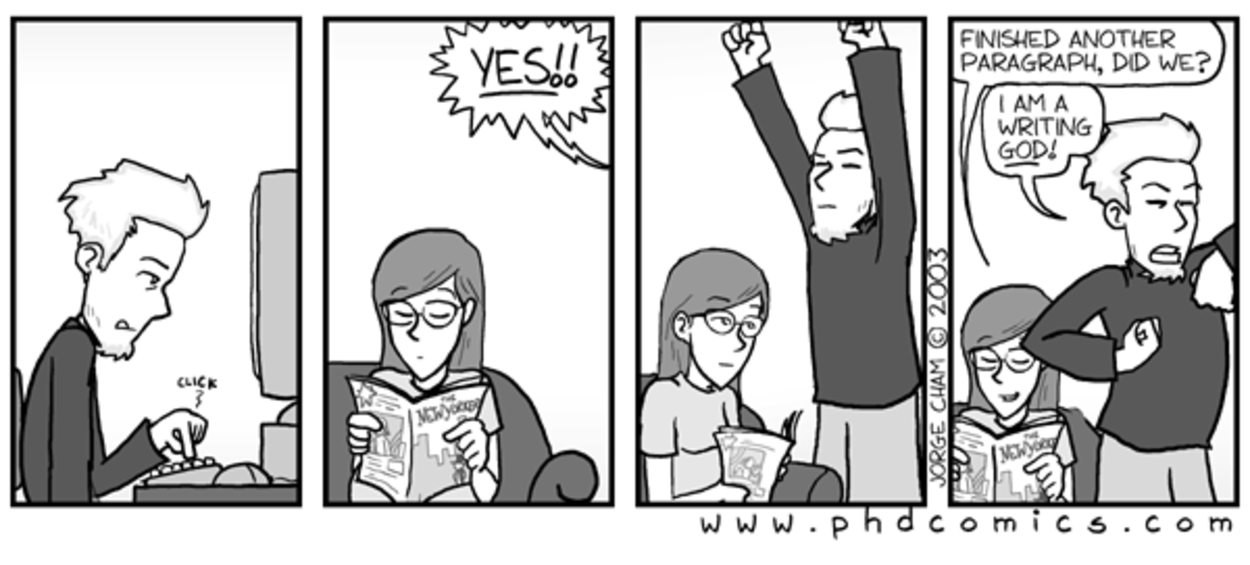
\includegraphics[width=\textwidth,keepaspectratio]{appendices/assets/comic}
\caption[Dissertation Writing Comic]{A Dissertation Writing Comic (from www.phdcomics.com).}
\label{fig:comic}
\end{figure}

\LaTeX{} is capable of using images in PDF, JPG and PNG format.

\subsection{Other Useful Commands}

There are some additional commands created to keep the formatting separated from the content, which we document below.

\texttt{\textbackslash keyword} -- Used to highlight keywords. For example, this is \keyword{somekeyword} (the command that produces this output is \texttt{\textbackslash keyword\{somekeyword\}}).

\texttt{\textbackslash tabhead} -- Used to highlight table headers. 

\texttt{\textbackslash code} -- Used to output code. For example, this \code{statement is formatted as code} (the command that produces this output is \texttt{\textbackslash code\{...\}}).

\texttt{\textbackslash file} -- Used to highlight files. For example, this is \file{somefilename} (the command that produces this output is \texttt{\textbackslash file\{somefilename\}}).

\texttt{\textbackslash option} -- Used to highlight options. For example, this is \option{someoption} (the command that produces this output is \texttt{\textbackslash option\{someoption\}}).

%----------------------------------------------------------------------------------------

\section{Sectioning and Subsectioning}

You should break your dissertation up into nice, bite-sized sections and subsections. \LaTeX{} automatically builds a table of Contents by looking at all the \texttt{\textbackslash chapter\{\}}, \texttt{\textbackslash section\{\}}  and \texttt{\textbackslash subsection\{\}} commands you write in the source.

The Table of Contents should only list the sections to three (3) levels. A \texttt{\textbackslash chapter\{\}} is level zero (0). A \texttt{\textbackslash section\{\}} is level one (1) and so a \texttt{\textbackslash subsection\{\}} is level two (2). In your dissertation it is likely that you will even use a \code{subsubsection\{\}}, which is level three (3). The depth to which the Table of Contents is formatted is set within \file{tmdei-style.cls}. If you need this changed, you can do it in \file{main.tex}.

%----------------------------------------------------------------------------------------

\section{Algorithms}

 \LaTeX{}  has several packages for typesetting algorithms in form of ''pseudocode''. In this template, we suggest the use of the \code{algorithm} environment with the \code{algpseudocode} package. 
More information about algorithms can be found at \url{https://en.wikibooks.org/wiki/LaTeX/Algorithms}.

Algorithm~\ref{alg:euclid} shows Euclid's algorithm that computes  Greatest Common Divisor (GCD) of two integer numbers.

\begin{algorithm}[b]
\caption{Euclid’s algorithm}
\label{alg:euclid}
\begin{algorithmic}[1]
\scriptsize

\State \textbf{Input}: Two integer numbers, $a$ and $b$
\State \textbf{Output}: GCD of $a$ and $b$
\State
\Procedure{Euclid}{$a,b$}\Comment{The GCD of $a$ and $b$}
\State $r\gets a\bmod b$
\While{$r\not=0$}\Comment{We have the answer if $r$ is $0$}
\State $a\gets b$
\State $b\gets r$
\State $r\gets a\bmod b$
\EndWhile
\State \textbf{return} $b$\Comment{The GCD is $b$}
\EndProcedure

\end{algorithmic}
\end{algorithm}

Here it is the \LaTeX{} text for the ''pseudocode'' algorithm presented in  Algorithm~\ref{alg:euclid}.

\begin{verbatim}
\begin{algorithm}
\caption{Euclid’s algorithm (pseudocode)}
\label{alg:euclid}
\begin{algorithmic}[1]
\scriptsize

\State \textbf{Input}: Two integer numbers, $a$ and $b$
\State \textbf{Output}:  Greatest Common Divisor (GCD) of $a$ and $b$
\State
\Procedure{euclid}{$a,b$}\Comment{The GCD of $a$ and $b$}
\State $r\gets a\bmod b$
\While{$r\not=0$}\Comment{We have the answer if $r$ is $0$}
\State $a\gets b$
\State $b\gets r$
\State $r\gets a\bmod b$
\EndWhile
\State \textbf{return} $b$\Comment{The GCD is $b$}
\EndProcedure

\end{algorithmic}
\end{algorithm}
\end{verbatim}

\texttt{\textbackslash listofalgorithms} command generates a list of all algorithms. This command is called in the \file{frontmatter.tex} file. Therefore, if there is no algorithm in the dissertation, this command must be removed (or commented) from such file.

\section{Source Code}
Sometimes there is the need to present programming source code snippets.
The \code{listings} package  is a powerful way to get nice source code highlighting in \LaTeX{}. It supports various programming languages, like Java (selected as the default language in this template), C, and many others.

Listing~\ref{lst:euclid_java} and Listing~\ref{lst:euclid_c} show the source code of the Euclid's algorithm, written in Java and C, respectively.

\begin{minipage}{\linewidth}
\lstinputlisting[
    language=Java,
    caption=Euclid's algorithm (Java).,
    label=lst:euclid_java
]{appendices/assets/euclid.java}
\end{minipage}

\begin{minipage}{\linewidth}
\lstinputlisting[
    language=C, 
    caption=Euclid's algorithm (C).,
    label=lst:euclid_c,
    numbers=none
]{appendices/assets/euclid.c}
\end{minipage}

Here it is the \LaTeX{} text for both listings. Note that we encapsulate the listings inside a \texttt{\textbackslash minipage} so that the listing does note break across pages.
Using the \texttt{\textbackslash lstinputlisting} command, the source code must be written in a separate file. In these two cases, both files are in \path{appendices/assets} directory.

\begin{verbatim}
\begin{minipage}{\linewidth}
\lstinputlisting[
    language=Java,
    caption=Euclid's algorithm (Java).,
    label=lst:euclid_java
]{appendices/assets/euclid.java}
\end{minipage}

\begin{minipage}{\linewidth}
\lstinputlisting[
    language=C,
    caption=Euclid's algorithm (C).,
    label=lst:euclid_c,
    numbers=none
]{appendices/assets/euclid.c}
\end{minipage}

\end{verbatim}
As it can be seen from the text above, there are a lot of parameters that can be specified, like programming language (\verb|language|), numbering, etc.   
More information about listings can be found at 
\url{https://en.wikibooks.org/wiki/LaTeX/Source_Code_Listings} and 
\url{http://texdoc.net/texmf-dist/doc/latex/listings/listings.pdf}.


\verb|\listoflisting| command generates a list of all source code listings. This command is called in the \file{frontmatter.tex} file. Therefore, if there are no listings in the dissertation, this command must be removed (or commented) from such file.

\section{The Portable Graphics Format}
The \gls{PGF} and a number of packages built on top of \gls{PGF} (such as TiKZ and PGFPLOTS) enable producing high quality graphical elements for your document. 
 
\subsection{TiKZ}
TikZ is built on top of PGF and allows you to create sophisticated graphics using \LaTeX{} commands. According to its author, Till Tantau~\footnote{Available online at \url{ftp://ftp.di.uminho.pt/pub/ctan/graphics/pgf/base/doc/pgfmanual.pdf}},  "\textit{What is TikZ? Basically, it just defines a number of \TeX{} commands
that draw graphics.}". With TikZ it is possible to accurately position picture elements, use \LaTeX{} fonts, incorporate mathematical typesetting, and use other \LaTeX{} features in your drawings.

The TikZ package defines the \verb|tikzpicture| environment that is required to draw a graphic. 
This environment must be inserted into a \verb|figure| environment when numbering and caption are required.
Figure~\ref{fig:tikz} shows a simple use of TiKZ, for which the \LaTeX{} source is as follows.

\begin{verbatim}
\begin{figure}[t]
\centering

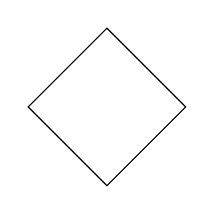
\begin{tikzpicture}
% Define four points
\coordinate (P0) at (1,0);
\coordinate (P1) at (0,1);
\coordinate (P2) at (-1,0);
\coordinate (P3) at (0,-1);
% Draw the diamond
\draw (P0)--(P1)--(P2)--(P3)--cycle;
\end{tikzpicture}

\caption{Using TiKZ for drawing pictures.}
\label{fig:tikz}
\end{figure}
\end{verbatim}

\begin{figure}[htb]
\centering

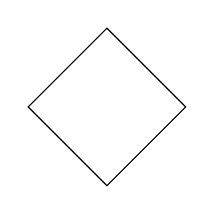
\begin{tikzpicture}
% Define four points
\coordinate (P0) at (0,0);
\coordinate (P1) at (1,0);
\coordinate (P2) at (0,1);
\coordinate (P3) at (-1,0);
\coordinate (P4) at (0,-1);
% Draw the diamond
\draw (P1)--(P2)--(P3)--(P4)--cycle;
\end{tikzpicture}

\caption{Using TiKZ for drawing pictures.}
\label{fig:tikz}
\end{figure}


A great amount of examples are available at \url{http://www.texample.net/tikz/examples/}. 
More information about TiKZ can be found at 
\url{https://en.wikibooks.org/wiki/LaTeX/PGF/TikZ} and 
\url{ftp://ftp.di.uminho.pt/pub/ctan/graphics/pgf/base/doc/pgfmanual.pdf}.

\subsection{PGFPLOTS}

PGFPLOTS provides tools to draw high quality plots, and is based on TiKZ. To use PGFPLOTS in the dissertation you need to use \verb|\usepackage{pgfplots}| (in \file{main.tex}).
To guarantee compatibility you need to specify \verb|\pgfplotsset{compat=<version>}|.
You can choose the \verb|version| ().
In this case, it is recommended to choose \verb|newest|. The choice \verb|compat=newest| means "I do not care if my old figures change in appearance after the next version upgrade".

Here it is the \LaTeX{} text for create the graph presented in Figure~\ref{fig:pgfplots}.
\begin{verbatim}
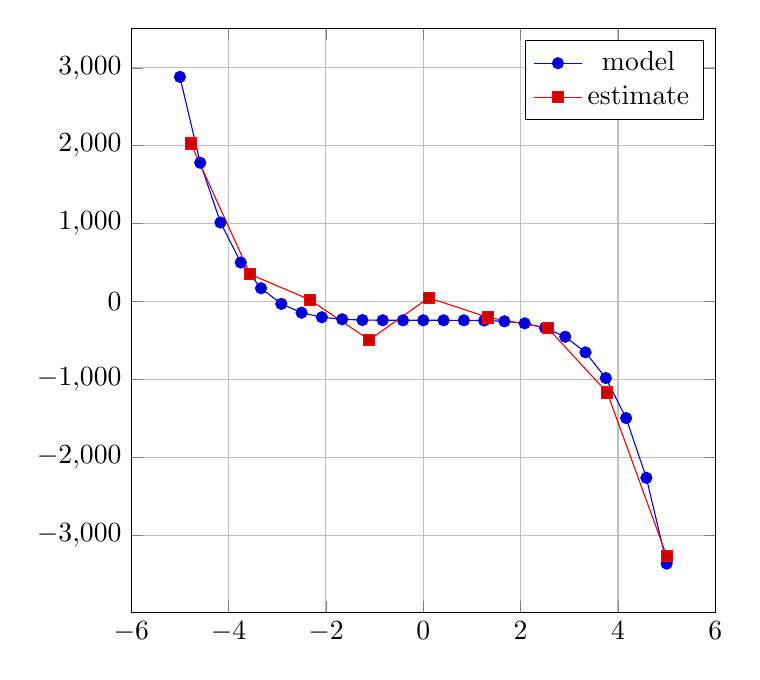
\begin{tikzpicture} 
	\begin{axis}[ height=9cm, width=9cm, grid=major, ] 
		\addplot {-x^5 - 242}; 
		\addlegendentry{model}
		\addplot coordinates { 
			(-4.77778,2027.60977) 
			(-3.55556,347.84069) 
			(-2.33333,22.58953) 
			(-1.11111,-493.50066) 
			(0.11111,46.66082) 
			(1.33333,-205.56286) 
			(2.55556,-341.40638) 
			(3.77778,-1169.24780) 
			(5.00000,-3269.56775) 
		}; 
		\addlegendentry{estimate} 
	\end{axis} 
\end{tikzpicture}
\end{verbatim}

Figure~\ref{fig:pgfplots} shows an example of a graph created using PGFPLOTS functions.

\begin{figure}[htb]
\centering
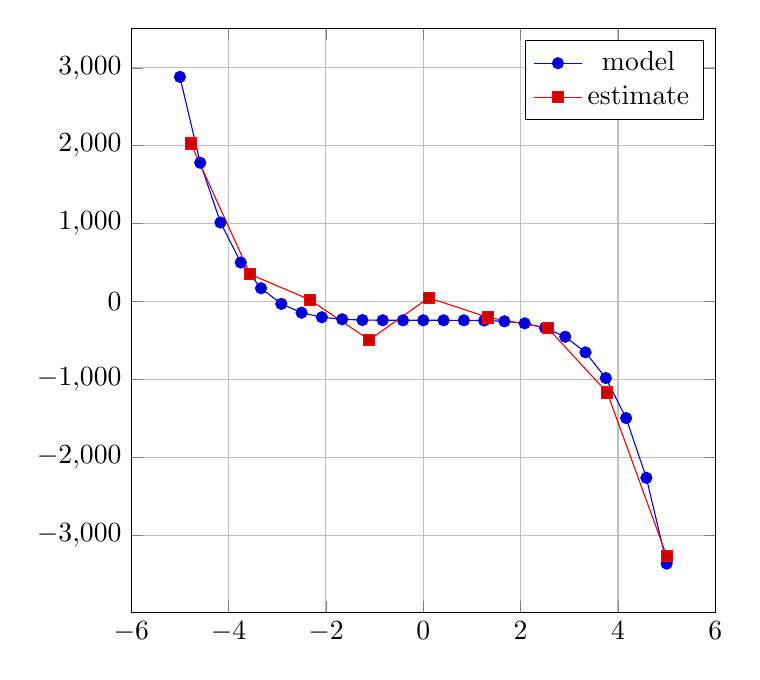
\begin{tikzpicture} 
	\begin{axis}[ height=9cm, width=9cm, grid=major, ] 
		\addplot {-x^5 - 242}; 
		\addlegendentry{model}
		\addplot coordinates { 
			(-4.77778,2027.60977) 
			(-3.55556,347.84069) 
			(-2.33333,22.58953) 
			(-1.11111,-493.50066) 
			(0.11111,46.66082) 
			(1.33333,-205.56286) 
			(2.55556,-341.40638) 
			(3.77778,-1169.24780) 
			(5.00000,-3269.56775) 
		}; 
		\addlegendentry{estimate} 
	\end{axis} 
\end{tikzpicture}
\caption{Using PGFPLOTS for drawing a graph.}
\label{fig:pgfplots}
\end{figure}

A great amount of examples are available at \url{http://pgfplots.sourceforge.net/gallery.html}. 
More information about TiKZ can be found at 
\url{http://pgfplots.sourceforge.net/pgfplots.pdf}.


\section{Handling Acronyms Automatically}
When writing a dissertation you need to define acronyms.
According to Wikipedia~\footnote{Accessed in 16 of December of 2015} \textit{"An acronym is an abbreviation used as a word which is formed from the initial components in a phrase or a word."} and
\textit{"Acronyms are used most often to abbreviate names of organizations and long or frequently referenced terms."}.
Typically, an acronym is a pronounceable word, which may already exist or it can be an invented word. 

The use of acronyms imposes two rules: (i) an acronym must be defined in the text during the first appearance of the phrase or word and (ii) the document must have a list of all acronyms alphabetically sorted. In \LaTeX{} this is provided by a package called \verb|\usepackage{glossaries}| that simplifies the use of acronyms. 

Included in this dissertation template there is a file called \file{glossary.tex} (in folder \file{frontmatter}), where all acronyms must be written in the form:
\begin{verbatim}
\newacronym{label}{abbrv}{full}
\end{verbatim}
where \verb|label| is the unique label identifying the acronym, \verb|abbrv| is the abbreviated form of the acronym and \verb|full| is the expanded text (word or phrase). This is an example of defining three acronyms:
\begin{verbatim}
\newacronym{RTS}{RTS}{Real-Time System}
\newacronym{GPOS}{GPOS}{General Purpose Operating System}
\newacronym{RTOS}{RTOS}{Real-Time Operating System}
\end{verbatim}

In order to use the features of the \verb|\usepackage{glossaries}|, you have only to use \verb|\gls{label}| command in the text. 
Using this command the acronym will be defined in the first appearance in the text and it will be listed in a list.
For instance, writing this \LaTeX{} text:
\begin{verbatim}
Linux is not a \gls{RTOS} but it is a \gls{GPOS}. 
VxWorks is a \gls{RTOS}, so it is not a \gls{GPOS}.
\end{verbatim}

outputs the following text: 

Linux is not a \gls{RTOS} but it is a \gls{GPOS}. VxWorks is a \gls{RTOS}, so it is not a \gls{GPOS}.

More information about acronyms can be found at 
\url{https://en.wikibooks.org/wiki/LaTeX/Glossary}.

%----------------------------------------------------------------------------------------

\section{In Closing}

You have reached the end of this mini-guide. You can now rename or overwrite this pdf file and begin writing your own \file{.tex} files and the rest of your dissertation. The easy work of setting up the structure and framework has been taken care of for you. It's now your job to fill it out!

Good luck and have lots of fun!

\begin{flushright}
Guide written by ---\\
Sunil Patel: \href{http://www.sunilpatel.co.uk}{www.sunilpatel.co.uk}\\
Vel: \href{http://www.LaTeXTemplates.com}{LaTeXTemplates.com}
\end{flushright}

%\input{appendices/appendixB}
%\input{appendices/appendixC}


%----------------------------------------------------------------------------------------
%	DOCUMENT END
%----------------------------------------------------------------------------------------

\end{document}
